
As outlined in section \ref{chap_mh_sampler}, the Metropolis Hastings Algorithm can be defined by its posterior probability and $Q(\Theta, \tilde{\Theta})$. The former can be computed recursively as shown in section \ref{chap_math_approach}; so $Q$ remains to be defined.

\textit{Symmetric Proposals}, i.e. proposals where $Q(\Theta, \tilde{\Theta}) = Q(\tilde{\Theta}, \Theta)$, are commonly employed. In absence of prior information indicating otherwise, this choice is natural as it does not arbitrarily favour some parameters over others. A common choice for a symmetric proposal is the normal distribution $\mathcal{N}(0, \sigma^2)$ for some $\sigma > 0$. 


\subsubsection*{Autocorrelation}
The choice of $\sigma$ directly influences the auto correlation the chain's samples will exhibit and hence the effective sample size. In particular, small values of $\sigma$ lead to proposals which are always very close to the current sample, incurring a high auto correlation. On the other hand, if $\sigma$ is too great, then the newly proposed value is likely to be extreme and hence unlikely. This makes the new sample very likely to be rejected. Rejection leads to strings of identical values, which are of course perfectly auto correlated.

Figures \ref{fig:sticky_chain} and \ref{fig:unsticky_chain} show two chains sampled with different choices of $\sigma$ for the same data and proposal distribution. They clearly illustrate how a $\sigma$ chosen too big can lead to poor behaviour of the resulting chain. 


\subsubsection*{Exploration of Search Space}
Small $\sigma$ lead to local suggestions; hence, multi-modal distributions are unlikely to be explored as the chain gets ''stuck'' in local maxima. A commonly used technique known as ''Simulated Annealing'' circumvents this phenomenon by decreasing $\sigma$ in the course of time. In the beginning, chains are then able to explore the search space, whereas later on with a small $\sigma$, they are also likely to zero in on the sought value. 

Please note that in Bayesian Inference, we are interesting in sampling a \textit{distribution} instead of a \textit{point estimate}. Hence, $\sigma$ cannot not be chosen arbitrarily small. 

\begin{figure}
	\begin{subfigure}[b]{0.9\textwidth}
		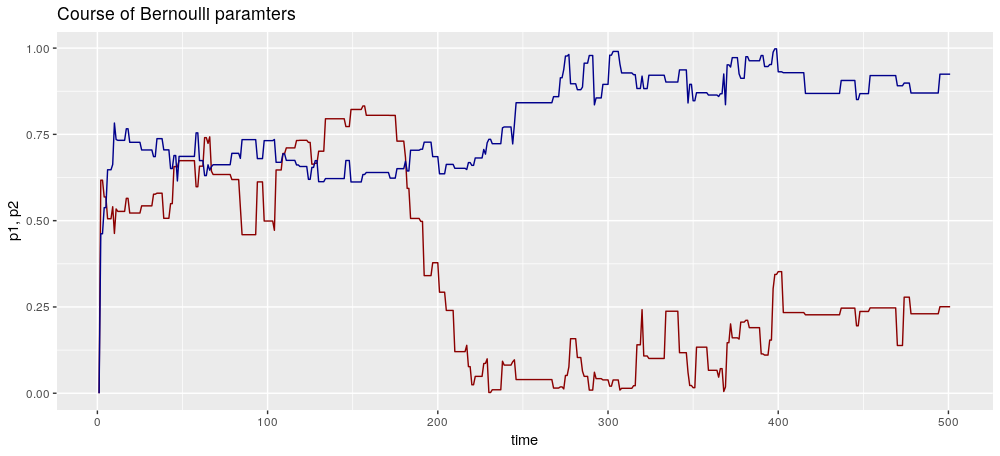
\includegraphics[width=\linewidth]{./img/sticky_chain.png}
		\caption{}
		\label{fig:sticky_chain}
	\end{subfigure}\\
	\begin{subfigure}[b]{0.9\textwidth}
		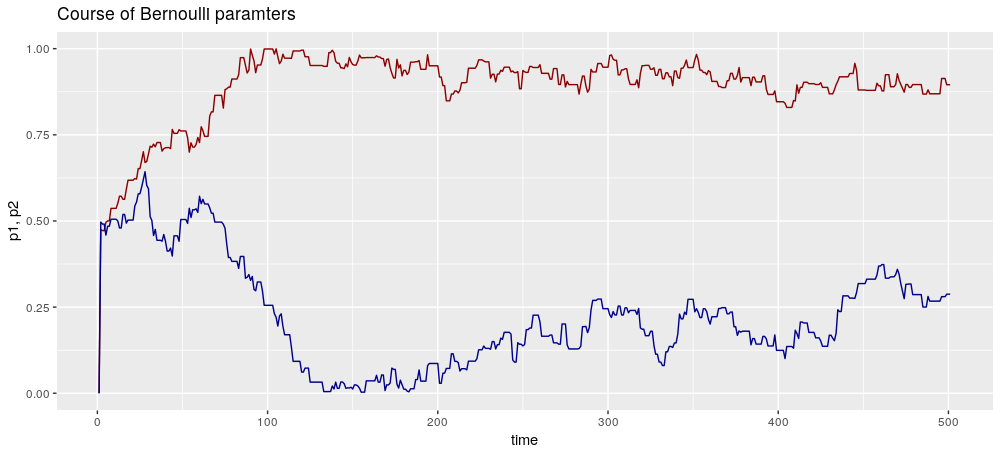
\includegraphics[width=\linewidth]{./img/unsticky_chain.png}
		\caption{}
		\label{fig:unsticky_chain}
	\end{subfigure}
	\caption{In figure \ref{fig:sticky_chain}, the path of the Bernoulli paramters of a Metropolis-Hastings chain with proposals $\mathcal{N}(0, 0.08^2)$ is shown; \ref{fig:unsticky_chain} uses proposals from $\mathcal{N}(0, 0.03^2)$. We can clearly see that the chain in \ref{fig:sticky_chain} is very ''stick'', i.e. often the chain rests with the current sample. On the other hand, the steps its Metropolis-Hastings sampler takes are usually greater than those of the not so sticky chain \ref{fig:unsticky_chain}. } 
\end{figure}


For these reasons, it is important to choose $\sigma$ wisely. Indeed, Johansen \cite{mcnotes} suggests to tweak $\sigma$ such as to obtain an acceptance rate of $0.44$ in the 1-dimensional case and $0.28$ in the multi-dimensional case. Often, those optimisations are performed manually by trial \& error; however, \cite{christen2010} suggests an algorithm adapting $\sigma$ automatically which appears to work well for many practical examples. 


\subsubsection{Modification of acceptance criterion}
As our algorithms work in log space, we modify the acceptance criterion as follows:
\codeBox{Metropolis-Hastings Acceptance Criterion in Log Space}{
	\begin{enumerate}
		\item Let 
		\begin{align}
		\tilde{\alpha} := min \Bigg\{ 0,  log\left( \tip{\tp} \, Q(\tp, \Theta) \right) - log\left( \tip{\Theta} \, Q(\Theta, \tp) \right) 			
		\Bigg\}
		\label{alphaSamplingStep}
		\end{align}
		\item Draw $u \sim U[0, 1]$
		\item If $log(u) \leq \tilde{\alpha}$, accept $\tp$ (i.e. set $\Theta_{t+1} = \tp$), otherwise reject it (i.e. $\Theta_{t+1} = \Theta_t$). 
	\end{enumerate} 
}

\subsection{Constrained Parameters}
For our purposes, $\Theta$ contains $\Gamma, \delta$ and a parameterisation of the states' distributions. Those are typically Bernoulli or Poisson distributions. 

All of those parameters are constrained:
\begin{itemize}
	\item $0 \leq \delta_i \leq 1$ with $\sum \delta_i = 1$ \\
	\item $0 \leq \Gamma_{j, i} \leq 1$ with $ \sum\limits_{i=1}^m \Gamma_{j, i} = 1$ \\
		for all $ 1 \leq j \leq m$
	\item $ 0 \leq p \leq 1$ for Bernoulli distributions or $\lambda \geq 0$ for Poisson distributions
\end{itemize}

When choosing a new proposal $\tilde{\Theta}$ from the current sample $\Theta$, with a step sampled from a normal distribution, it is not immediately clear how to ensure that the new proposal satisfies the constraints. 

\subsubsection*{Natural and Working Parameters}
A common approach to deal with this is to apply transformations such as the $log$-transformation. For instance, if a parameter is constrained to $[0,1]$, we could work in a transformed space instead. 
For instance, if our algorithm was to suggest values in $(-\infty, \infty)$ (so-called \textit{working parameters}), we could apply the log-transformation to map those values into $[0,1]$ (so-called \textit{natural parameters}); this would ensure that all new proposals are valid from a model point of view. 

However, the steps are usually normally distributed in the space of the natural parameters and it is unclear what the distribution of a random variable $X$ would be s.t. $exp(X) \sim \mathcal{N}(0, \sigma)$. 




\subsubsection*{''Bumping'' of Parameters}
Let $p \in [0,1]$ be a parameter and $s: [0,1] \rightarrow \R$ be a function mapping $p$ to a new proposal. Then we draw new samples as follows:
\codeBox{Bumping of parameters}{
	\begin{algorithmic}
			\State $\tilde{p} \gets s(p)$
			\If {$\tilde{p} \in [0, 1]$}
				\State $p \gets \tilde{p}$
			\ElsIf{$min\{ abs(p - 0), abs(1-p) \} < 1$}
				\If {$\tilde{p} < 0$ }
					\State $p \gets - \tilde{p}$
				\Else
					\State $p \gets 1 - (\tilde{p} - 1)$
				\EndIf
			\EndIf
	\end{algorithmic}
}
We note the following:
\begin{enumerate}
	\item the interval can easily be generalised
	\item the proposal is symmetric
	\item if the proposed new sample is farther than $1$ away from both $0$ and $1$, the new sample is rejected. The variance of the proposal distribution should be chosen small s.t. this case becomes unlikely.
\end{enumerate}



\subsubsection{Drawing from a constrained distribution}
% source: https://stats.stackexchange.com/questions/142999/simulate-from-a-truncated-mixture-normal-distribution/143011#143011
We would prefer to directly draw a parameter from a distribution which respects the constraints the parameter is subject to over rejecting or bumping a parameter after it has been drawn. 

One way to do so is to use a \textit{truncated normal distribution}.
Let us denote the normal distribution, truncated to the interval $[a, b]$ with $X \sim \mathcal{N}_a^b(\mu, \sigma^2)$. 

\begin{lemma}
	The cdf of $X$ is \\
	\begin{align*}
	F(x) = \begin{cases}
		0	& x \leq  a \\
		\frac{
			\Phi\left( \frac{x - \mu}{\sigma} \right)
			- \Phi\left(\frac{a - \mu}{\sigma}\right)
		}{
		\Phi\left(\frac{b - \mu}{\sigma}\right)
		- \Phi\left(\frac{a - \mu}{\sigma}\right)
		}
	    & \, \text{otherwise}
		\end{cases}
	\end{align*}
	\label{lem:cdf}
\end{lemma}

\begin{proof}
	Let $\tilde{X} \sim \mathcal{N}(\mu, \sigma^2)$. \\
	Then we have 
	\begin{align*}
		F_{ \tx \, | \, \tx \in [a, b]}(x) &= \frac{\uP{\tx < x \cap \tx \, \in \, [a, b]} }{\uP{\tx \, \in \, [a, b]}} \\
		&= \frac{\uP{\nt{\tx} < \nt{x} \cap \nt{\tx} \, \in \, \left[\nt{a}, \nt{b} \right]} }{\uP{\nt{\tx} \, \in \, [\nt{a}, \nt{b}]}} \\
		&\overset{x \, \geq \, a}{=} \frac{\nd{x} - \nd{a}}{\nd{b} - \nd{a}}
	\end{align*}
\end{proof}

\begin{theorem}[The Inversion Method]
Let $X \sim F$ where $F$ is some cdf and let $F^{-1}$ be the inverse\footnote{or if the inverse does not exist, the pseudo-inverse} of $F$. 
Then
\[
F_X^{-1}(U[0, 1]) \sim X
\]
\end{theorem}

Lemma \ref{lem:cdf} provides us with the cdf of a truncated normal distribution; using the inversion method, we can thus sample from a truncated normal distribution. Please note that neither the cdf nor the inverse are available in analytical forms; still, numerical approximations are readily available in R.

Note that sampling methods which do not involve $\Phi$ or $\Phi^{-1}$ are also available; notably, \cite{Robert95simulationof} proposes a method based on Rejection-Sampling. 
 

% R code for sampling:
% x = qnorm(  pnorm(a,mu,sigma) + runif(1)*(pnorm(b,mu,sigma) - pnorm(a,mu,sigma))  




